\scanpage{224}
% printed form
% Reverse-side computer print visible through the paper; read in reflected order.
\texttt{\unsure{//***} CRAY2 \unsure{1324} \illegible{2}}
\figure{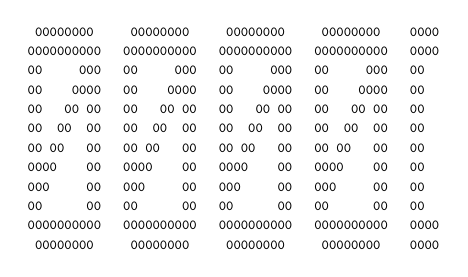
\begin{tikzpicture}[x=1pt,y=1pt,every node/.style={anchor=west,inner sep=0pt,font=\tiny\ttfamily}]
\node at (0,0) {~00000000~~~~~00000000~~~~~00000000~~~~~00000000~~~~\unsure{0000}};
\node at (0,-7) {0000000000~~~0000000000~~~0000000000~~~0000000000~~~\unsure{0000}};
\node at (0,-14) {00~~~~~000~~~00~~~~~000~~~00~~~~~000~~~00~~~~~000~~~\unsure{00}};
\node at (0,-21) {00~~~~0000~~~00~~~~0000~~~00~~~~0000~~~00~~~~0000~~~\unsure{00}};
\node at (0,-28) {00~~~00~00~~~00~~~00~00~~~00~~~00~00~~~00~~~00~00~~~\unsure{00}};
\node at (0,-35) {00~~00~~00~~~00~~00~~00~~~00~~00~~00~~~00~~00~~00~~~\unsure{00}};
\node at (0,-42) {00~00~~~00~~~00~00~~~00~~~00~00~~~00~~~00~00~~~00~~~\unsure{00}};
\node at (0,-49) {0000~~~~00~~~0000~~~~00~~~0000~~~~00~~~0000~~~~00~~~\unsure{00}};
\node at (0,-56) {000~~~~~00~~~000~~~~~00~~~000~~~~~00~~~000~~~~~00~~~\unsure{00}};
\node at (0,-63) {00~~~~~~00~~~00~~~~~~00~~~00~~~~~~00~~~00~~~~~~00~~~\unsure{00}};
\node at (0,-70) {0000000000~~~0000000000~~~0000000000~~~0000000000~~~\unsure{0000}};
\node at (0,-77) {~00000000~~~~~00000000~~~~~00000000~~~~~00000000~~~~\unsure{0000}};
\end{tikzpicture}}

\figure{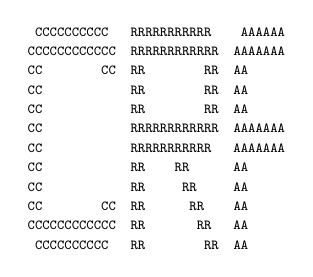
\begin{tikzpicture}[x=1pt,y=1pt,every node/.style={anchor=west,inner sep=0pt,font=\tiny\ttfamily}]
\node at (0,0) {~CCCCCCCCCC~~~RRRRRRRRRRR~~~~AAAAAA};
\node at (0,-7) {CCCCCCCCCCCC~~RRRRRRRRRRRR~~AAAAAAA};
\node at (0,-14) {CC~~~~~~~~CC~~RR~~~~~~~~RR~~AA};
\node at (0,-21) {CC~~~~~~~~~~~~RR~~~~~~~~RR~~AA};
\node at (0,-28) {CC~~~~~~~~~~~~RR~~~~~~~~RR~~AA};
\node at (0,-35) {CC~~~~~~~~~~~~RRRRRRRRRRRR~~AAAAAAA};
\node at (0,-42) {CC~~~~~~~~~~~~RRRRRRRRRRR~~~AAAAAAA};
\node at (0,-49) {CC~~~~~~~~~~~~RR~~~~RR~~~~~~AA};
\node at (0,-56) {CC~~~~~~~~~~~~RR~~~~~RR~~~~~AA};
\node at (0,-63) {CC~~~~~~~~CC~~RR~~~~~~RR~~~~AA};
\node at (0,-70) {CCCCCCCCCCCC~~RR~~~~~~~RR~~~AA};
\node at (0,-77) {~CCCCCCCCCC~~~RR~~~~~~~~RR~~AA};
\end{tikzpicture}}

\diagram{\(\begin{array}{llllll}
\texttt{****A}&\texttt{START}&\texttt{JOB}&\texttt{\unsure{1324|324}}&\texttt{CRAY2}&\texttt{ROOM}\ \unsure{1}\\
\texttt{****A}&\texttt{START}&\texttt{JOB}&\texttt{1324}&\texttt{CRAY2}&\texttt{ROOM}\ 1\\
\texttt{****A}&\texttt{START}&\texttt{JOB}&\texttt{1324}&\texttt{CRAY2}&\texttt{ROOM}\ 1\\
\texttt{****A}&\texttt{START}&\texttt{JOB}&\texttt{1324}&\texttt{CRAY2}&\texttt{ROOM}\ 1\\
\texttt{****A}&\texttt{START}&\texttt{JOB}&\texttt{1324}&\texttt{CRAY2}&\texttt{ROOM}\ 1\\
\texttt{****A}&\texttt{START}&\texttt{JOB}&\texttt{1324}&\texttt{CRAY2}&\texttt{ROOM}\ 1
\end{array}\)}

\texttt{DERNIERE MISE A JOUR \unsure{DE|DU} JOURNAL : \unsure{11-08-82}}\\
\texttt{ATTENTION \unsure{.............}}

\texttt{\unsure{J|1}\hspace{1em}1. UNE MODIFICATION SYSTEME NOUS CONTRAINDRA A DETRUIRE}\\
\texttt{J\hspace{2em}LE CONTENU DU DISQUE SPOOL LE MARDI 17 AOUT A \unsure{8|4} HEURES}\\
\texttt{J\hspace{2em}VEUILLEZ RECUPERER VOS SORTIES EN ATTENTE AVANT CETTE}\\
\texttt{J\hspace{2em}DATE. MERCI DE VOTRE COMPREHENSION.}\\
\texttt{J\hspace{1em}2. UN ARRET EXCEPTIONNEL POUR PREPARER L'ARRIVEE DE NOUVE\unsure{L}}\\
\texttt{J\hspace{2em}UNITES AURA LIEU DU VENDREDI 20 AOUT A 17H 30 AU LUNDI}\\
\texttt{J\hspace{2em}23 AOUT A 8H.}

% archive sheet number: 223

